% --------------------------------------------------------------
% This is all preamble stuff that you don't have to worry about.
% Head down to where it says "Start here"
% --------------------------------------------------------------
 
\documentclass[12pt]{article}
 
\usepackage[margin=1in]{geometry} 
\usepackage{amsmath,amsthm,amssymb}
\usepackage{xcolor}
\usepackage{listings}
\usepackage{graphicx}
\usepackage{hyperref}
\usepackage{listings}
\graphicspath{{../plots/}}

\newcommand{\N}{\mathbb{N}}
\newcommand{\Z}{\mathbb{Z}}
 
\newenvironment{theorem}[2][Theorem]{\begin{trivlist}
\item[\hskip \labelsep {\bfseries #1}\hskip \labelsep {\bfseries #2.}]}{\end{trivlist}}
\newenvironment{lemma}[2][Lemma]{\begin{trivlist}
\item[\hskip \labelsep {\bfseries #1}\hskip \labelsep {\bfseries #2.}]}{\end{trivlist}}
\newenvironment{exercise}[2][Exercise]{\begin{trivlist}
\item[\hskip \labelsep {\bfseries #1}\hskip \labelsep {\bfseries #2.}]}{\end{trivlist}}
\newenvironment{problem}[2][Problem]{\begin{trivlist}
\item[\hskip \labelsep {\bfseries #1}\hskip \labelsep {\bfseries #2.}]}{\end{trivlist}}
\newenvironment{question}[2][Question]{\begin{trivlist}
\item[\hskip \labelsep {\bfseries #1}\hskip \labelsep {\bfseries #2.}]}{\end{trivlist}}
\newenvironment{corollary}[2][Corollary]{\begin{trivlist}
\item[\hskip \labelsep {\bfseries #1}\hskip \labelsep {\bfseries #2.}]}{\end{trivlist}}

\newenvironment{solution}{\begin{proof}[Solution]}{\end{proof}}
\definecolor{codegreen}{rgb}{0,0.6,0}
\definecolor{codegray}{rgb}{0.5,0.5,0.5}
\definecolor{codepurple}{rgb}{0.58,0,0.82}
\definecolor{backcolour}{rgb}{0.95,0.95,0.92}

\lstdefinestyle{mystyle}{
    backgroundcolor=\color{backcolour},   
    commentstyle=\color{codegreen},
    keywordstyle=\color{magenta},
    numberstyle=\tiny\color{codegray},
    stringstyle=\color{codepurple},
    basicstyle=\ttfamily\footnotesize,
    breakatwhitespace=false,         
    breaklines=true,                 
    captionpos=b,                    
    keepspaces=true,                 
    numbers=left,                    
    numbersep=5pt,                  
    showspaces=false,                
    showstringspaces=false,
    showtabs=false,                  
    tabsize=2
}
\lstset{style=mystyle}
\begin{document}
 
% --------------------------------------------------------------
%                         Start here
% --------------------------------------------------------------
 
\title{Assignment 1: gem5 Tutorial}
\author{Arpit Prasad\\ 
COL718 - Architecture for High Performance Computers}

\maketitle

\section{Overview}

In this assignment we perform sweep analysis of systems by varying the type of CPU, CPU frequency and Memory Configuration. For this assignment we have used the 
following type for each of the mentioned variables:
\begin{enumerate}
    \item CPU Types:
    \begin{enumerate}
        \item TIMING: In Order Execution
        \item O3: Out of Order Exection
    \end{enumerate}
    \item CPU Frequency: A sweep from 0.6GHz to 3.3GHz in steps of 0.2GHz
    \item Memory Configuations:
    \begin{enumerate}
        \item Single Channel DDR3 1600MHz
        \item Single Channel DDR4 2400MHz
        \item High Bandwidth Memory 
    \end{enumerate}
\end{enumerate}

Following are the plots and variation of performances obtained in the sweep.

\section{Matrix Multiplication}

Reference for matrix Multiplication was taken from the following https://www.akkadia.org/drepper/cpumemory.pdf

Here we perform block wise multiplication. This allows an entire block to be loaded onto the cache at once, and hence lesser miss rate.

The binary produced from this code was done with following command

\begin{lstlisting}[language=sh, frame=single, numbers=left, caption={Shell Script used to obtain binary}]
    g++ -O3 mm.c -o mm
\end{lstlisting}

for agressive optimisations.

The size of the matrices was assumed to be 100x100



\section{Performance Metrics}
\noindent The following is the overview of the performance metrics that are used to analyse the performance of a code with respect to a Model

Note, the performance metrics are evaluated on SE mode (System Exection Mode)
\begin{enumerate}
    \item IPC: Instructions Per Cycle, indicating the throughput of the system
    \item Simulation Seconds: Amount of time in seconds to simulate a binary on the simulated device
    
\end{enumerate}

\section{Plots}

\subsection{IPC vs Frequency}
First we keep Memory Configuation fixed and vary CPU Types and then CPU Type fixed and vary Memory Configuation
\subsubsection{CPU Variation}
From Fig. 1 the IPC remains nearly constant for both the types of CPU. This is because
IPC is the measure of instructions per cycle. Therefore, as frequency increases
the number of instruction per second increases and and the same time number of cycles per
second. Therefore their division remains constant.

\noindent We can also see O3 being out of order has higher IPC than TIMING which has in order exection

\begin{figure}[h]
    \centering
    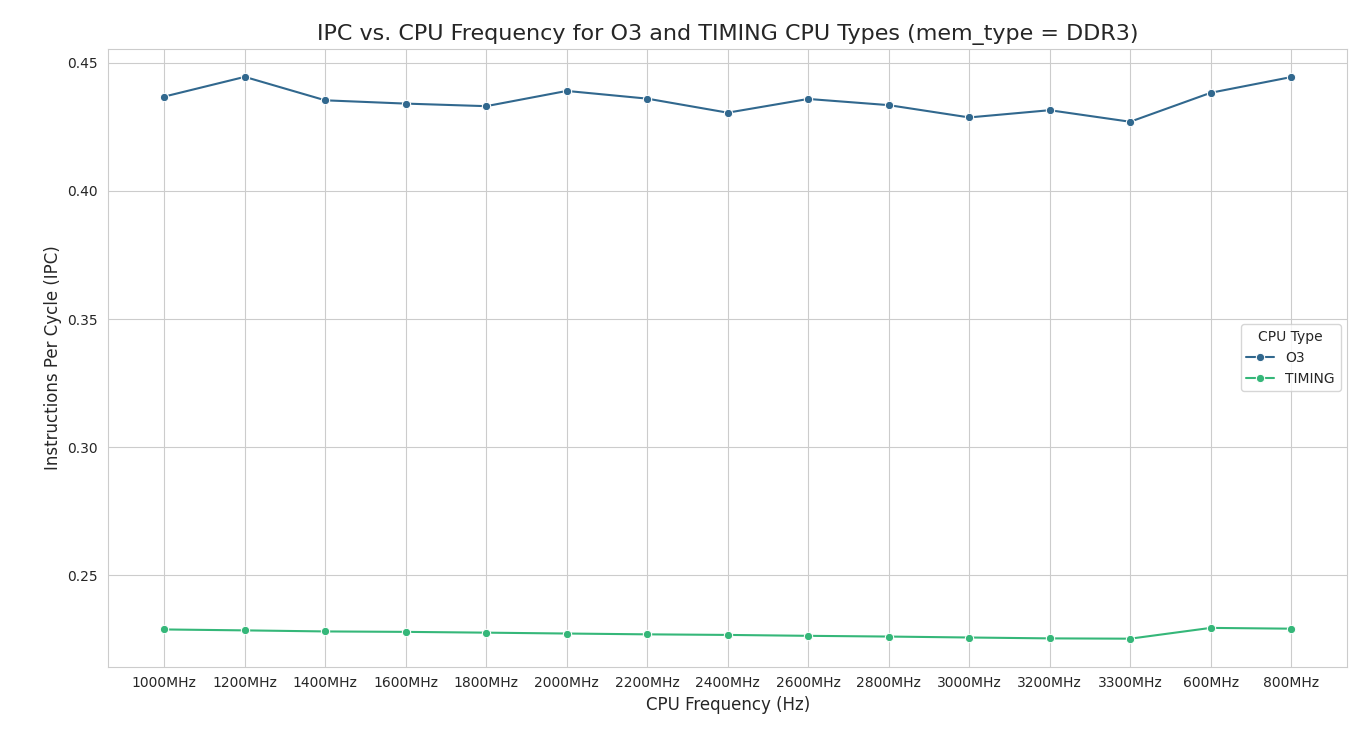
\includegraphics[width=0.8\textwidth]{ipc_vs_feq_line.png}
    \caption{Variation of IPC when changing the frequency of the chipset, given a particular Memory Configuation}
\end{figure}

\subsubsection{Memory Configuation Variation}

From Fig. 2 we again notice the value of IPC almost remains constant. (Note the scale of the graph makes it appear visually to vary highly.)
Similar arguments as mentioned above apply here. HBM should technically be 
faster than DDR3, however this cannot be reflected from the IPC vs Frequency graph due to 
seconds cancelling on the division of Instructions/sec and Cycles/sec
\begin{figure}
    \centering
    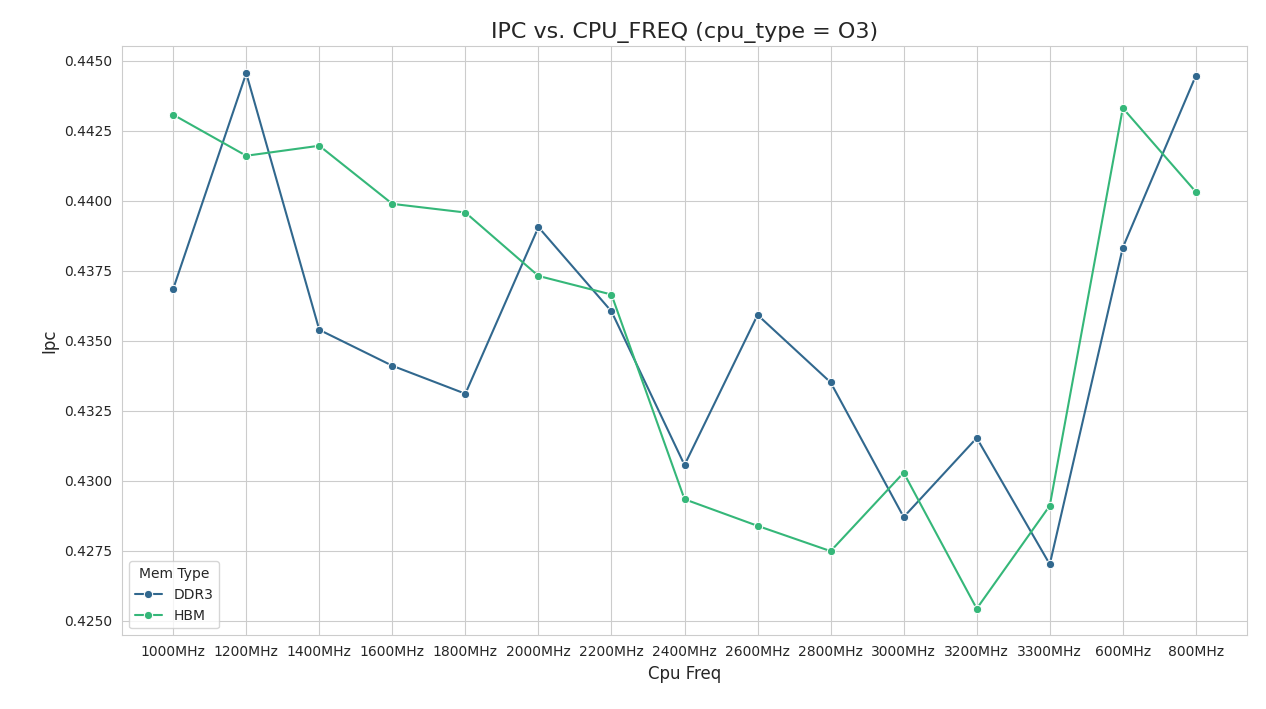
\includegraphics[width=0.8\textwidth]{ipc_vs_freq_mem.png}
    \caption{Variation of IPC when changing frequency of the chipset, given a pparticular CPU Type}
\end{figure}

\subsection{Simulation Seconds vs Frequency}
Again, we follow the same pattern, i.e., first we keep Memory Configuation fixed and 
vary CPU Types and then CPU Type fixed and vary Memory Configuation.

\subsubsection{CPU Variation}
From Fig. 3, the variation we observe a downward trend in the graph. Since as the frequency increases the 
amount of time taken for simulation decreases, since the number of instructions exected per second increases

Again CPU Type O3 has smaller simulation time for a given frequency since it operates
on out of order execution. Whereas, TIMING operates in order execution

\begin{figure}[h!]
    \centering
    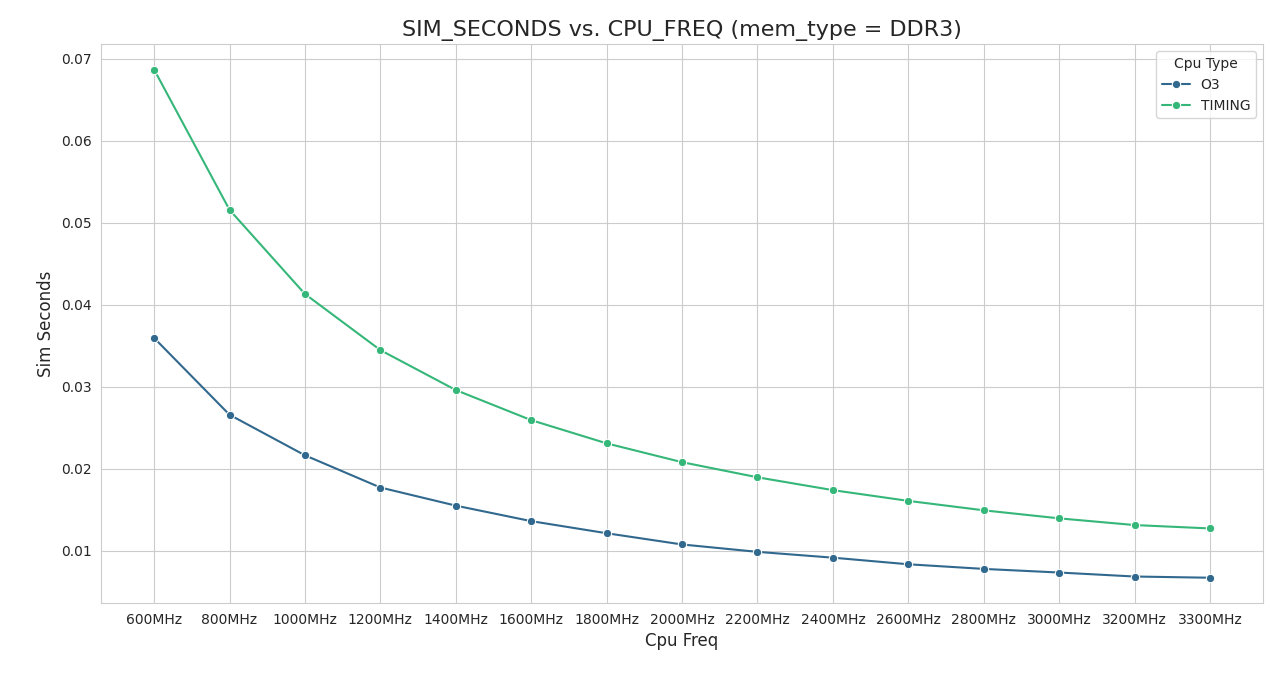
\includegraphics[width=0.8\textwidth]{sims_vs_freq.png}
    \caption{Simulation Seconds vs Frequency, given a Memory Configuation}
\end{figure}


\subsubsection{Memory Configuration Variation}

From Fig. 4 we again observe a downward sloping curve. However, here we observe
the exact similar values of the different types of memory configurations. For different types of memory units we obsever similar values of simulation times given a frequency because as sweep through the frequency, either the max frequency of transfer of data from memory unit limits the cpu frequency when it is greater than memory's frequency or vice versa. Therfore at frequency lower than memory frequency, data transfers occur at cpu frequency. At higher cpu frequency, the data transfer is limited by the max frequency of memory

\begin{figure}[h!]
    \centering
    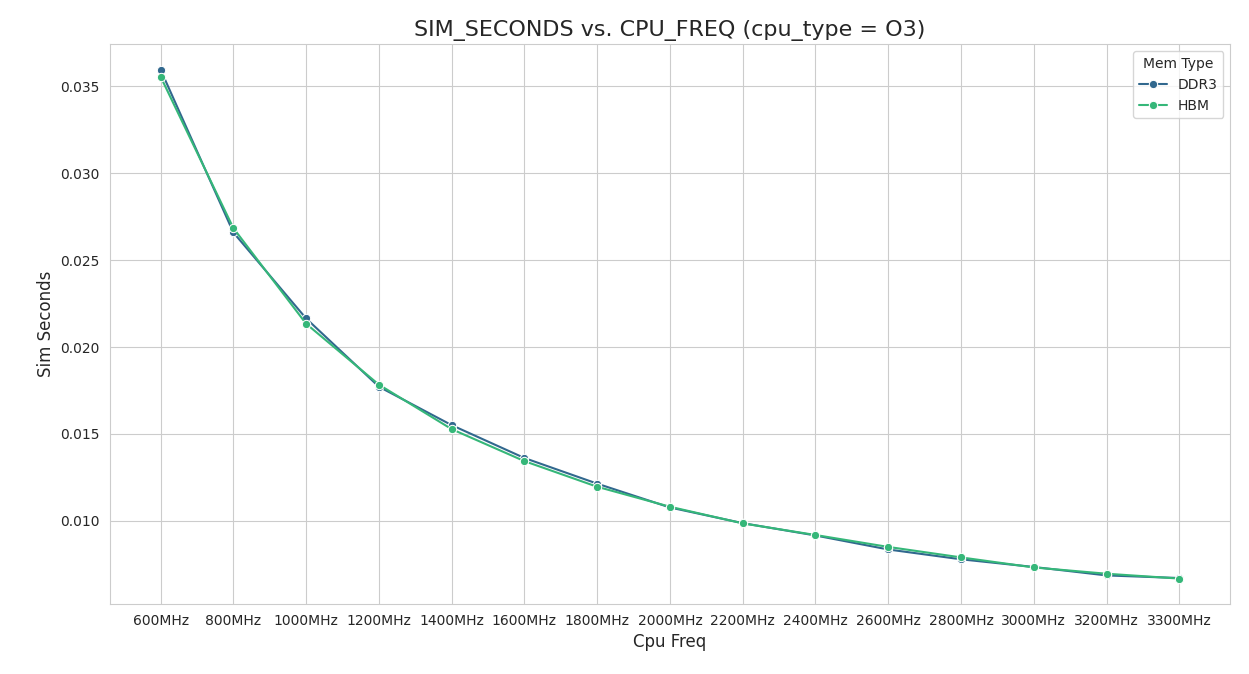
\includegraphics[width=0.8\textwidth]{sims_vs_freq_mem.png}
    \caption{Simulation Seconds vs Frequency, given a CPU Type}
\end{figure}

\subsection{Latency}

We consider the average read and write Latencies of the systems, using a memory of Single Channel DDR3
\begin{table}[h]
    \centering
    \caption{Variation of Latencies with CPU Types}
    \resizebox{1.1\linewidth}{!}{
    \begin{tabular}{|c|c|c|c|c|} % l: left, r: right, r: right alignment for the three columns
        \hline
        CPU Type & Order of Exection & Frequency & Read Latency (ticks / count) & Write Latency (ticks / count) \\
        \hline
        O3 & Out of Order & 600MHz & 27663.28 & 1020144433.51 \\
        
        TIMING & In Order & 600MHz & 29226.18 & 2080891024.17 \\
        \hline
        O3 & Out of Order & 800MHz & 28242.87 & 741798455.68 \\
        
        TIMING & In Order & 800MHz & 28712.47 & 1489806432.79 \\
        \hline
    \end{tabular}    }
\end{table}

From Table 1, clearly both the read and the write latencies are better for O3, which is executes instructions out of order.

Latencies do not show variation with increase in frequency since they are measured in ticks per count. As frequency increases the number of ticks per second and count per second both increase and hence their division remains nearly constant.

% --------------------------------------------------------------
%     You don't have to mess with anything below this line.
% --------------------------------------------------------------

\end{document}
